\documentclass[11pt]{article}
\usepackage[margin=0.75in]{geometry}            % See geometry.pdf to learn the layout options. There are lots.
\geometry{letterpaper}                                  % ... or a4paper or a5paper or ... 
%\geometry{landscape}                           % Activate for rotated page geometry
%\usepackage[parfill]{parskip}                  % Activate to begin paragraphs with an empty line rather than an indent
\usepackage{graphicx}                           % Use pdf, png, jpg, or eps§ with pdflatex; use eps in DVI mode
                                                                % TeX will automatically convert eps --> pdf in pdflatex                
\usepackage{amssymb}
\usepackage{upquote}

%-----------------------------------------------------------------------------
% Special-purpose color definitions (dark enough to print OK in black and white)
\usepackage{color}
% A few colors to replace the defaults for certain link types
\definecolor{orange}{cmyk}{0,0.4,0.8,0.2}
\definecolor{darkorange}{rgb}{.71,0.21,0.01}
\definecolor{darkgreen}{rgb}{.12,.54,.11}
%-----------------------------------------------------------------------------
% The hyperref package gives us a pdf with properly built
% internal navigation ('pdf bookmarks' for the table of contents,
% internal cross-reference links, web links for URLs, etc.)
\usepackage{hyperref}
\hypersetup{pdftex, % needed for pdflatex
  breaklinks=true, % so long urls are correctly broken across lines
  colorlinks=true,
  urlcolor=blue,
  linkcolor=darkorange,
  citecolor=darkgreen,
}


\title{Wireless Sensor Network Project\\
  Stat 222, Spring 2016}

\author{
  Jamie Palumbo\\
  \texttt{jcpalumbo3}
}


\begin{document}
\maketitle

\abstract{\textit{A Macroscope in the Redwoods} utilized a wireless sensor network to record 44 days in the life of a 70-meter tall redwood tree in Sonoma California during the early summer. Climate variables including temperature, humidity, incident photosynthetically active solar radiation (PAR), and reflected PAR were recorded every 5 minutes from nodes placed approximately every 2 meters in space. The project that follows gives an overview of the data collection process, suggests graphical improvements to the paper, and describes the data cleaning process and the exploratory data analysis that followed.}


\section{Introduction}

This report investigates the data collected from a wireless sensor network to gain insights into the environmental dynamics of a coastal redwood tree. The study deployed 33 nodes, shielding a suite of climate sensors from environmental damage, in order to study temporal and spatial trends through multi-dimensional data analysis. Section 2 provides an overview of the data collection process, the data cleaning process, and the data exploration that followed. Section 3 provides a graphical critique of the figures presented in the original paper and suggests improvements to better display the findings. Section 4 presents the top findings from the exploratory data analysis that was performed. A brief discussion and conclusion follow. 

\section{The Data}


\subsection{Data Collection}
The researchers deployed a wireless sensor network to measure spatial and temporal climate variables including temperature, humidity, incident photosynthetically active solar radiation (PAR), and reflected PAR.  The data was collected for two redwood trees (referred to as interior and edge) in Sonoma California every 5 minutes over a 44 day span in the early summer. Specifically, the first reading was recorded on Tuesday, April 27, 2004, and the last was recorded on Thursday, June 10, 2004. The early summer was chosen as it contains the most dynamic microclimatic variation. Nodes were placed at a vertical distance of 15 meters to 70 meters from the ground with a roughly 2 meter gap between nodes. The majority of the nodes were placed on the west side of the tree since it had a thicker canopy to protect the nodes from environmental elements. Finally, the nodes were placed 0.1-1.0 meters from the trunk to ensure that the measurements captured the microclimatic trends that affected the tree directly, not the broader climate. Overall, the maximum number of readings is 50,540 real-world data points per mote, or approximately 1.7 million data points for the 33 interior tree motes.  

\subsection{Data Cleaning}
In order to perform any analysis, the data required significant cleaning as there were several gross outliers, inconsistencies, and missing values as illustrated in Figure 1. Since the all file was comprised of the data collected from both the wireless network and the flash logs, I opted to clean the net and log files separately, combine them, and then remove any duplicate values.\\

\begin{figure}
  \centering
    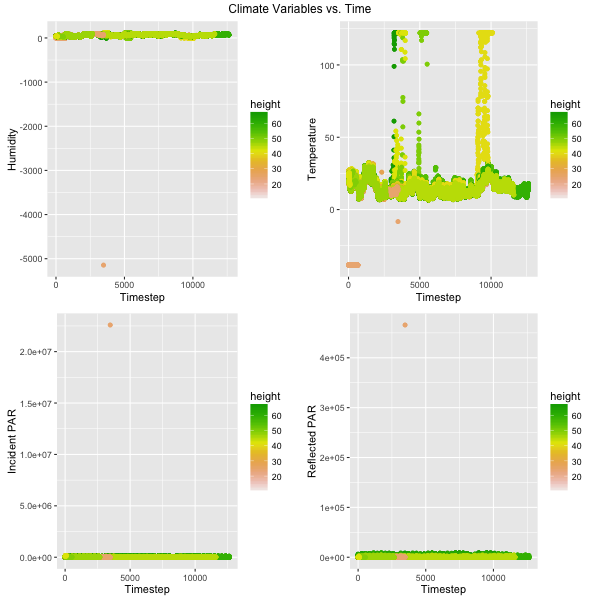
\includegraphics[width=\textwidth,height=14cm]{../graphs/figure2.png}
  \caption{Original Dataset}
  \label{fig:fig2}
\end{figure}

First, I looked at the net data. After collecting all the rows with missing values, I found that node 122 was entirely the culprit. I deleted this node since it suggested the sensors were not working properly. Next, I plotted humidity versus time, finding that nodes 78, 123, and 141 were attributed to the negative humidity readings while nodes 3, 118, and 145 were attributed to the very high positive readings. I deleted all but node 118 since the variables plotted against time exhibited very strange behavior and since the log file contained cleaner readings for these nodes. I then plotted temperature versus time. While nothing looked too unusual, I subsetted by the temperature readings greater than 30, concluding that nodes 119 and 127 might have just had a minor outlier or two. Adjusted humidity, incident PAR, and reflected PAR did not exhibit any unusual behavior when plotted against time so I moved onto voltage. I subsetted by the voltage readings greater than 1000, finding that nodes 134 and 135 had very large flatlined values. Knowing that the rest of their readings were appropriate, I set their voltages equal to NA.\\
\\
Having removed the outliers from the net data, I moved onto cleaning the log data. I first plotted humidity versus time, finding that nodes 29, 198, and 65535 were attributed to the negative humidity readings. I set these outlying values to NA since the majority of the readings seemed to be correct. Nothing seemed too unusual in regards to temperature, adjusted humidity, incident PAR, and reflected PAR. However, I did remove PAR readings for node 40 since it was displaying erratic behavior. Finally, I removed several flatlined voltage values.\\
\\
After cleaning the net and log datasets, I combined the two datasets and created a new column that counted the number of duplicated nodeid and epoch pairs. I first removed all exact duplicated rows. Next, I focused on nodeid and epoch pairs that were repeated twice, deleting both values from the data set and inserting a row that took the mean of the climate variables. Finally, I repeated the process for nodeid and epoch pairs that were repeated three times. The cleaned climate variables can be seen in Figure 2.  
\begin{figure}
  \centering
    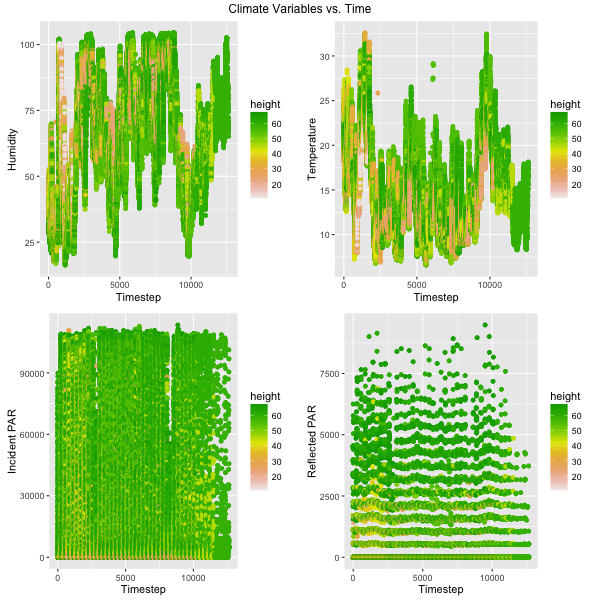
\includegraphics[width=\textwidth,height=14cm]{../graphs/figure1.png}
  \caption{Cleaned Dataset}
  \label{fig:fig1}
\end{figure}

\subsection{Data Exploration}
Before beginning my exploratory data analysis, I left joined the cleaned dataset with the location variables, hoping to uncover an interesting relationship between the climate variables and the direction or height of the node. I focused on the interior tree since the summary statistics suggested that the edge tree had far fewer observations.\\
\\
The first step in my analysis was to gain a better understanding of the dataset. While cleaning the dataset, I had noticed that several plots did not include the entire epoch range. I further explored this notion by plotting a histogram of the counts over time. This will be explained in more detail in the findings section. I also plotted similar histograms for the log and net datasets individually, finding that the nodes lower in the tree tended to drop off more so than the higher nodes over time.\\
\\ 
I then plotted each variable over time, colored by height first and then direction. However, these plots are very difficult to discern patterns from since they are cluttered with so many observations. I decided to refine these plots by focusing on observations collected on a single day. Similar to the paper itself, I chose to focus on May 1st since it contained wide-ranging temperature and humidity readings. The patterns became much more evident. I found that humidity is higher closer to the ground than in the canopy while temperature, incident PAR, and reflected PAR are higher in the canopy than closer to the ground. Humidity peaked around 8 AM while temperature, incident PAR, and reflected PAR peaked between 12 and 2 PM. It was difficult to discern any patterns in regards to the direction. I then chose to refine these plots further by plotting the lowest, highest, and median height nodes. These plots displayed the aforementioned trends more clearly, even revealing that the lower nodes experienced a lag before displaying the same behavior as the highest node in terms of temperature and humidity as seen in Figure 3.\\


\begin{figure}
  \centering
    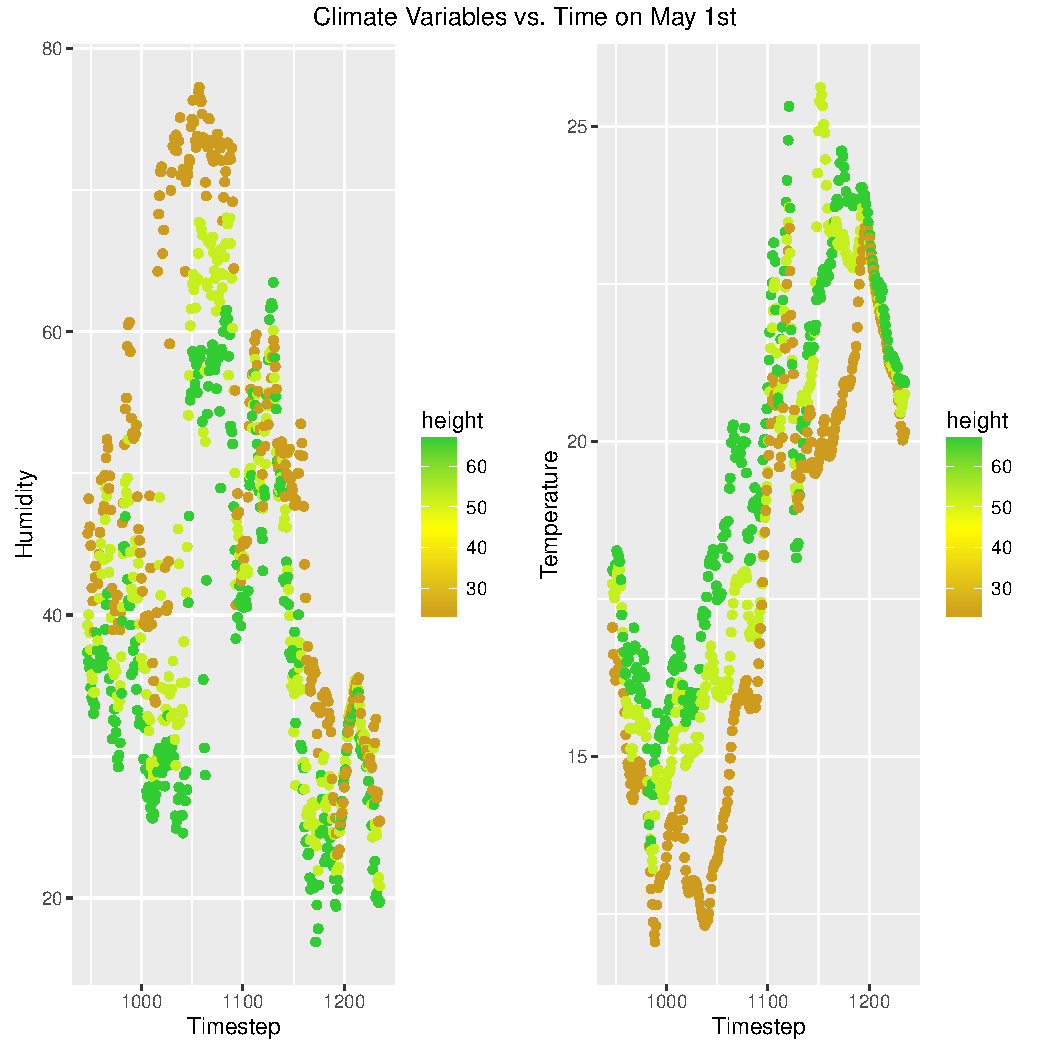
\includegraphics[width=\textwidth,height=14cm]{../graphs/figure3.pdf}
  \caption{Temperature and humidity against time on May 1st}
  \label{fig:find3}
\end{figure}

The final part of my exploratory analysis involved plotting the climate variables against temperature, colored by height, both overall and for May 1st. These plots showed similar patterns. Humidity showed a negative correlation with temperature, regardless of height, while the other variables showed very little correlation with temperature.  

\section{Graphical Critique}
While the graphics included in the paper do display some information well, there is much room for improvement. Let us first consider Figure 3 which makes use of the dataset cleaned by the researchers' outlier rejection method. In general, the information in these graphs do not adjust for the number of observations at each height. From the findings section below, we see that higher nodes tend to have more data than lower nodes which could potentially skew the results. 
\begin{enumerate}
\item[(a)]
Figure 3a attempts to display the distribution of the readings for all four climate variables. According to the paper, the main message of this graphic is to show that temperature and reflected PAR have a unimodal distribution while humidity and incident PAR have a bimodal distribution. However, it seems that the histograms use the default intervals which may provide a different story compared to a smaller bin size. I believe these graphics could be improved by decreasing the bin size, adding color to also show how height is distributed, removing the inner tick marks on the top and right of the graphs, and minimizing the whitespace in the PAR plots.  

\item[(b)]
Figure 3b attempts to find temporal trends and weather movement in the local microclimate by displaying the distribution of readings over time. However, there are so many outliers graphed that it is difficult to see any trends, especially for the PAR readings. It could be beneficial if the authors had graphed only the daytime readings for PAR since the nighttime readings are always zero. Additionally, the graphics would be more informative if they included height information in the form of color since height is incredibly correlated with these climate variables. This could have been accomplished using a line graph, colored by height. Finally, the x-axis is distracting and would look cleaner if the labels were rotated to display all the dates consistently. 

\item[(c)]
Figure 3c attempts to display the distribution of readings taken by each sensor at each height in order to show spatial trends. Again, PAR trends might be more evident if the authors only displayed daytime data. The trends in these graphs are not very evident and could be more obvious if the variables were plotted against time and colored by height. 

\item[(d)]
Figure 3d attempts to display the distribution of sensor reading differences from the mean. This is probably the most interesting of the four panels as it shows the range for each node and has very evident trends displayed. 

\end{enumerate}
The main goal of Figure 4 is to display a day in the life of a redwood by plotting each of the climate variables against time. The authors were attempting to show temporal trends but did not include height in the graphics. The top two line charts on the left make use of color, but it is ambiguous as to what the color represents. It seems to me that the colors represent the nodes, but they could have just as easily represented the different heights which would have resulted in no loss of spatial information. This use of color is also inconsistent with the bottom two graphs which are entirely in green. The graphs on the right display spatial location plotted against spatial gradients at a single moment in time. Not much information can be gleaned from these graphs since they do not display any trends. I am also uncertain as to why this time was chosen. In general, I believe these graphs could be improved by adding titles and legends so that the figures can stand on their own. Transparency or jittering of points would also help the reader better understand the information displayed.  

\section{Findings}


\subsection{First finding}

My first interesting finding involved the observation counts and frequencies over time. The left hand side plot of Figure 4 is a histogram which displays the number of observations in 100 epoch bins for each node height. The right hand side plot displays this same information in the form of frequencies. As illustrated in Figure 4, the majority of the nodes do not capture data covering the entire time range. At approximately 3000 epoch, a quarter of the observations fall off. At about 8000 epoch, we are left with about half of the observations. Then, at a little over 10000 epoch, we are left with only three nodes worth of observations. We also see that over time, the data is skewed towards nodes that are placed higher in the tree. This could significantly affect the interpretation of the results. 

\begin{figure}
  \centering
    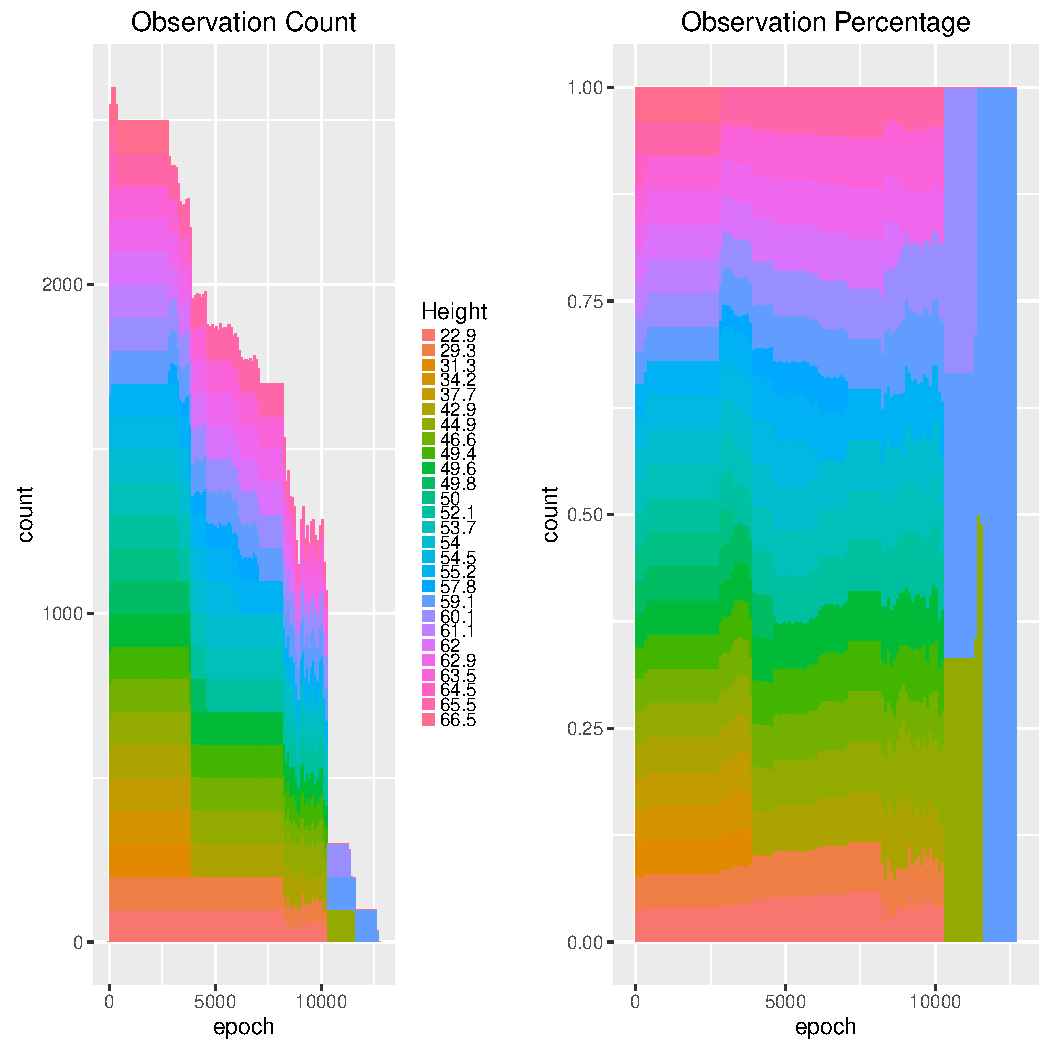
\includegraphics[width=\textwidth,height=14cm]{../graphs/finding1.pdf}
  \caption{Observation counts and frequencies over time and height}
  \label{fig:find1}
\end{figure}


\subsection{Second finding}

My second finding in Figure 5 plots humidity, temperature, incident PAR, and reflected PAR against time on May 1st. Similar to the authors, I chose May 1st since it had wide-ranging values for the climate variables. Each of these plots is colored by height, revealing important patterns. For example, we see that nodes placed higher in the canopy tend to have lower humidity readings than those placed lower to the ground. In contrast, nodes placed higher in the canopy tend to have higher temperature readings than those placed lower to the ground. We also see that incident and reflected PAR tend to be higher for nodes placer higher in the canopy as they are exposed to more sunlight. These observations confirm our hypotheses about climate variables in relation to height.  

\begin{figure}
  \centering
    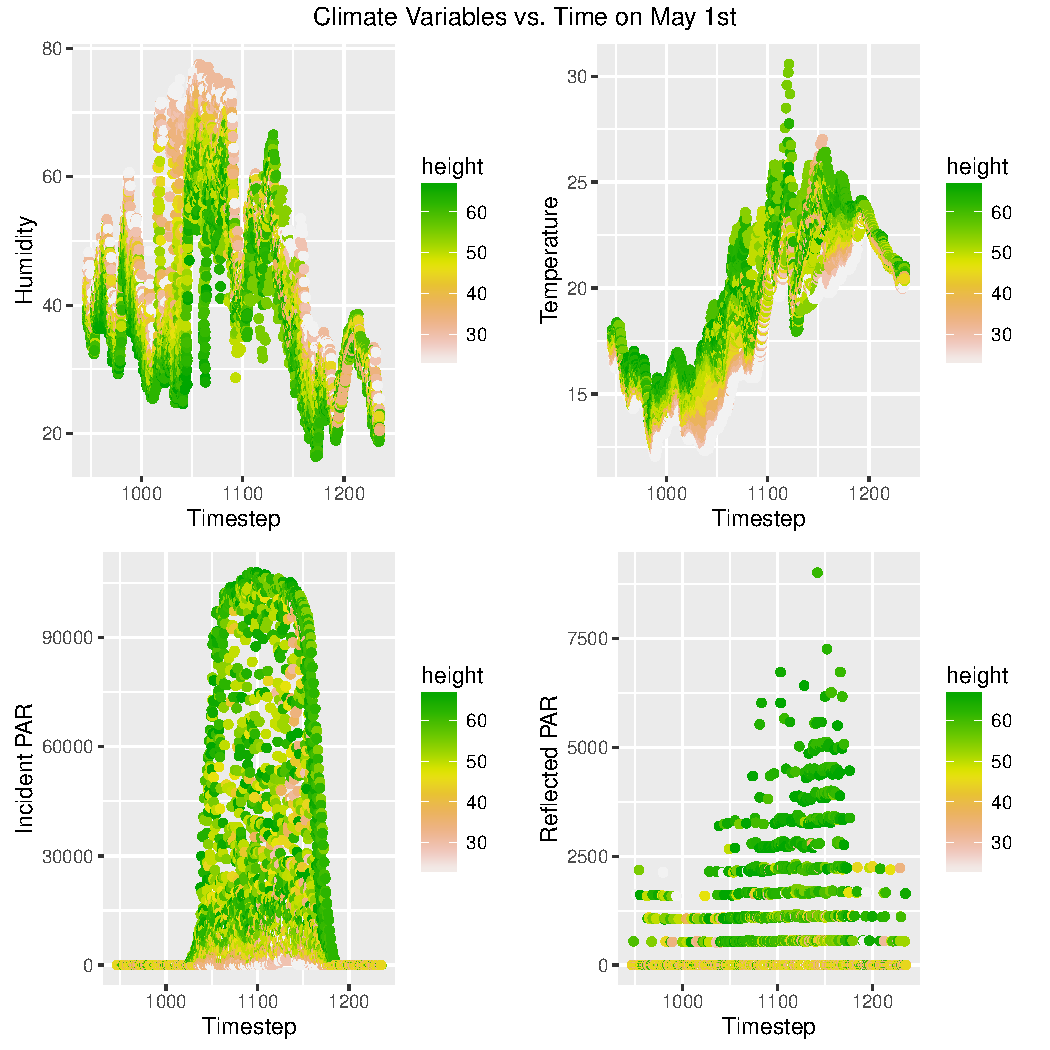
\includegraphics[width=\textwidth,height=14cm]{../graphs/finding2.pdf}
  \caption{Climate variables fluctuating over time on May 1st}
  \label{fig:find2}
\end{figure}


\subsection{Third finding}
My third and final finding in Figure 6 considers the relationship between humidity and temperature. I would have expected to see a different relationship between humidity and temperature at different heights due to varying amounts of sunlight and canopy coverage. However, this was not the case. The two variables display a negative correlation that is independent of height. 


\begin{figure}
  \centering
    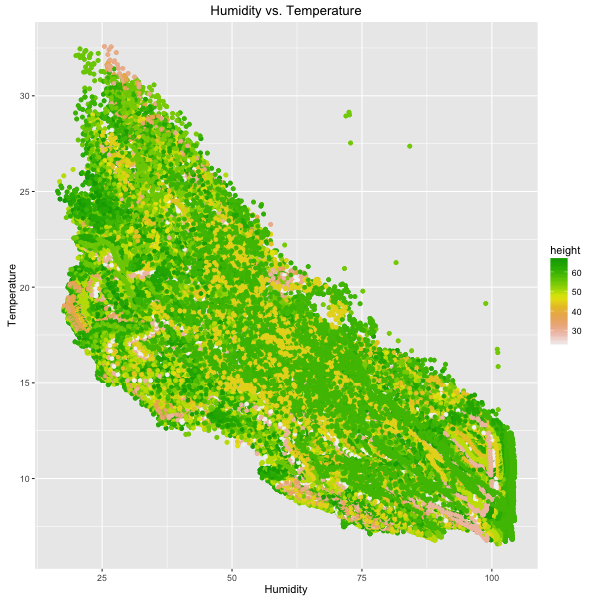
\includegraphics[width=12cm,height=10cm]{../graphs/finding3.png}
  \caption{Relationship between humidity and temperature}
  \label{fig:find3}
\end{figure}


\section{Discussion}
There were several lessons learned from working with the data from a wireless sensor network. Data from such large scale, multi-dimensional networks is oftentimes messy, inconsistent, and incomplete, requiring considerable data cleaning to get the data into a workable form. Additionally, such high dimensional datasets are difficult to visualize and interpret and should be considered from several different viewpoints to glean meaningful results. 

\section{Conclusion}
Wireless sensor networks enable researchers to collect large volumes of data over time. In this particular instance, data was collected from a coastal redwood to get a glimpse of the environmental dynamics experienced by the tree. However, properly cleaning the data without removing important information is a challenging task. It is also challenging to accurately display such large quantities of data to give a complete representation of the trends. Deliberate cleaning and data analysis techniques along with attention to detail in graphical illustrations can help collapse a multi-dimensional framework into a more tractable, meaningful form.   


% the `Acknowledgments` section is required if you discussed the project
% with anyone else.
%\section*{Acknowledgments}


\bibliographystyle{plain}
\bibliography{sensor}

\end{document}
